\section{RL Optimized Rule-based Agent}
\label{sec:rule-based_agent}

For the \textit{hit} and \textit{prepare} task defined in \ref{subseq:reward} a rule-based controller was implemented.
This controller was then optimized through PGPE \cite{PGPE} following the approach in \cite{PGPE_Likmeta}.

In this case the robot is controlled using the \textit{task space}, combining inverse kinematics and Anchored Quadratic Programming (AQP) \cite{baseline}.

The policy set was divided into 2 main branches that resemble the challenge tasks: hit and prepare. Each policy is
further divided into phases, common to both of them:
\begin{itemize}
    \item \textit{Adjustment}: move the end-effector on (i) the line linking the puck and the goal for the hit; (ii) the vertical line
    parallel to the short side, passing through the puck, for the prepare.
    \item \textit{Acceleration}: accelerate the end-effector and hit the puck. The hit policy hits the puck to score a goal, while
    the prepare one makes a more soft bump, in order to re-adjust the puck's position;
    \item \textit{Final}: this phase only applies to the hit policy. Here, the agent keeps hitting the puck making it reach a desired
    acceleration, then slowly stops the end-effector following a curved trajectory.
\end{itemize}

In particular, the hit policy computes two quantities, $d\beta$ and $ds$ in the following way:
\begin{equation*}
    d\beta = \left\{
        \begin{aligned}
            &(\theta_0 + \theta_1 \cdot t_{phase} \cdot dt) \cdot correction \quad & adjustment \text{ phase}\\
            &\frac{correction}{2}                                            \quad & acceleration \text{ phase}\\
            &(\theta_0 + \theta_1 \cdot dt) \cdot correction                 \quad & slow\text{-}down \text{ phase}
        \end{aligned}
    \right.
\end{equation*}

\begin{equation*}
    ds = \left\{
        \begin{aligned}
            &\theta_2                                                                    \quad & adjustment \text{ phase}\\
            &\frac{ds_{t-1} + \theta_3 \cdot t_{phase} \cdot dt}{radius + r_{mallet}}    \quad & acceleration \text{ phase}\\
            &constant                                                                    \quad & slow\text{-}down \text{ phase}
        \end{aligned}
    \right.
\end{equation*}

where $radius$ is the distance between the center of the puck and the end-effector, while $correction$ is always defined as:

\begin{equation*}
    correction = \left\{
        \begin{aligned}
            \beta - 90° \quad&y_{puck} \le 0 \\
            270° - \beta \quad&y_{puck} > 0
        \end{aligned}
    \right.
\end{equation*}

All the quantities appearing in the computation of $d\beta$ and $ds$ are explained graphically in Figure \ref{fig:polar_coordinates}

\begin{figure}
    \centering
    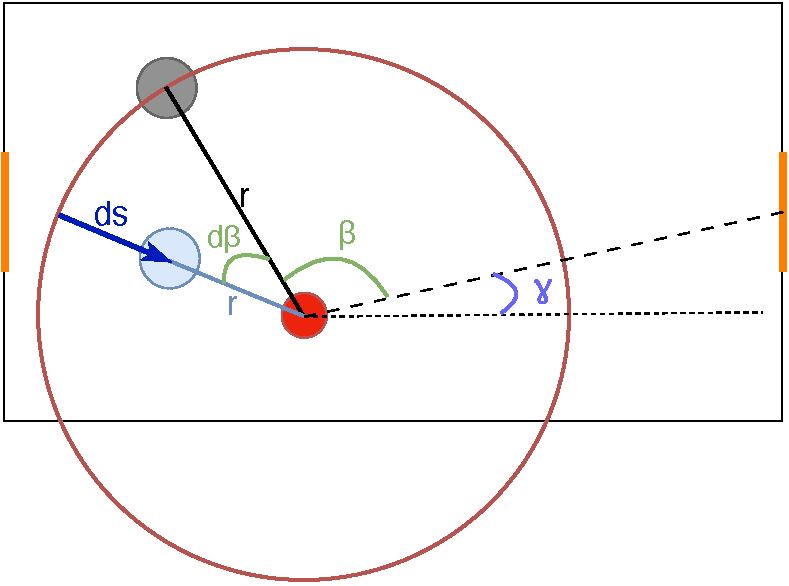
\includegraphics[width=0.5\textwidth]{Images/polar_coordinates.pdf}
    \caption{Polar coordinates used in the Rule-based controllers}
    \label{fig:polar_coordinates}
\end{figure}

